% Figure M6, generated by experiments/m6_pitprops.py.
\begin{figure}[t]
  \centering
  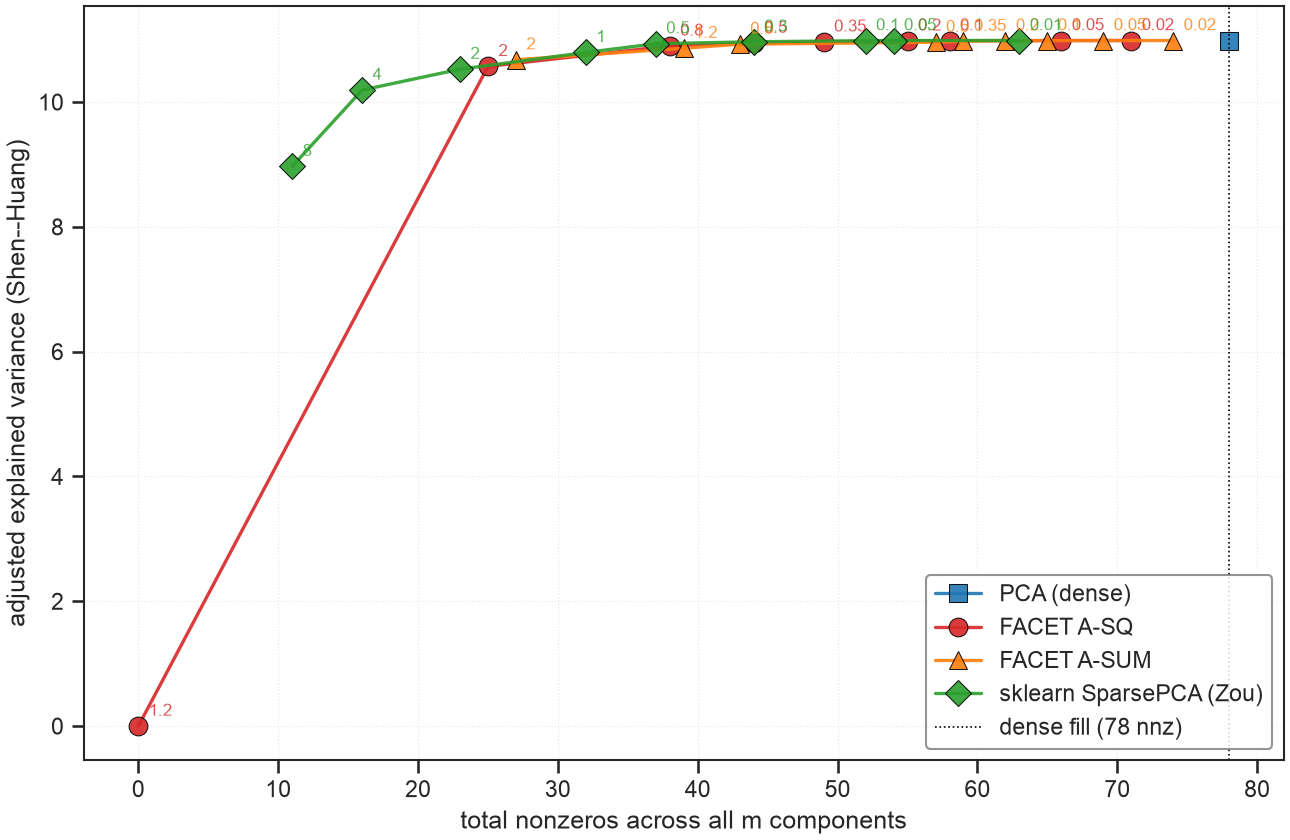
\includegraphics[width=0.92\linewidth]{../shared/figures/generated/m6_pitprops.png}
  \caption{\textbf{M6, classical sparse-PCA benchmark on Jeffers Pitprops} \citep{jeffers1967pitprops}; thirteen-variable correlation data, $m{=}6$ components. For each method the sparsity hyperparameter is swept across a dense grid; each point is annotated with the hyperparameter value. Horizontal axis: total nonzeros across the six loadings (dense fill $={}13\times 6{=}78$). Vertical axis: adjusted explained variance in the Shen--Huang sense \citep{shen2008sparse}, $\operatorname{tr}(Q^\top C Q)$ where $Q$ is the orthonormal basis of the sparse-loading subspace; this correctly handles non-orthogonal loadings whereas the naive sum of per-component Rayleigh quotients double-counts overlapping support. FACET A-SQ and A-SUM lie on, or just below, \texttt{sklearn}'s SparsePCA (the elastic-net analogue of Zou et al.~\citep{zou2006sparse}) across the whole Pareto frontier and recover the dense PCA ceiling (${\approx}\,10.986$) by $\mathrm{nnz}\!\approx\!60$. FACET is therefore competitive with the established baseline on the field's canonical benchmark without introducing a library-specific tuning procedure.}
  \label{fig:m6-pitprops}
\end{figure}
